\documentclass[12pt]{article}
\usepackage{lingmacros}
\usepackage{tree-dvips}
\usepackage{multicol}
\usepackage{graphicx}
\usepackage[section]{placeins}
\usepackage{hyperref}
\usepackage{caption}
\usepackage{listings}
\usepackage{indentfirst}


\hypersetup{
	colorlinks=true,
	linkcolor=blue,
	filecolor=magenta,      
	urlcolor=cyan,
}
\title{\Huge \bfseries \emph{Assignment 2}}
\author{Vathana Him}
\date{November 1, 2021}

\begin{document}
\maketitle
\section{Abstract}
\hspace*{5mm} The purpose of this assignment is to use the data of the image created from assignment 1 to build classification models in order to classify the choosen images. 
This assignment utilized images from UCI respository as sample datasets that will be used to train a machine learning model. 
Images that were processed represented three fruits spanish pear, fuji apple, watermelon. These images were labeled as Image0, Image1, and Image2 respectively. 
These labels was then encoded to take in the values of 0, 1, and 2. Two machine learning was used in order to classify these images. The Elastic
Net penalty was used to classify a two-class dataset and Random Forest classifier was used to classify a multi-class dataset. Prior to training the machine learning model,
additional methods were taken into account in feature selection and data scaling in order to reduce the size of the data and train the model with a sufficient outcome.
Finally, the results between the Elastic Net and Random Forest model was examined. 

\begin{multicols*}{2}
  \section{Task 1}
  \hspace*{5mm} In order to begin working on this project, there were python libraries that needed to be installed. Thus, the libraries that were used were pandas, sklearn, matplolib,
  and seaborn. The data for the images that were choosen was first divided into a test and train split. This test and train split divided the dataset for each
  respective images into a 80:20 ratio of train-test split. Then a histogram for each training and test sets were generated for the nonoverlapping and non overlapping images.
  Seaborn was primarly used for plotting histogram and scatterplot. The plot was created with a helper function created in the code that requires the input of
  a dataframe and two columns name in order to generate a plot. 
  
  \hspace*{5mm} The two features that were choosen for the histogram plots were features 54 and 56. In the non-overlapping images01, it is
  evident that features 54 and features 56 follows the same left skewed distribution based on 2.1 Figure 1. Based on 2.1 Figure 2, the test set of the non-overlapping images01,
  the distribution follow a similar left skewed distribution pattern. The mean for both the test and train set for non-overlapping images01 of features 54 
  and 56 were both 184 and 183 respectively. Thus, there was not a large deviation of mean from feature 54 and 56 from the train and test set of non-overlapping
  images01. Similary features 54 and 56 were also choosen to plot histograms for the non-overlapping dataset of images012. Based on 2.1 Figure 3 and Figure 4, 
  it can be concluded that the test and train set followed the same left skewed distribution pattern. The mean and variances of the respective train and test
  set did no vary to a large degree as their mean was 173 for all and their variances ranging from 1970 to 1980. This suggests that the testing and splitting 
  method for the non-overlapping images provided a good randomeses among the batches of dataset, which would help against any biases when training a machine learning
  model.

  \hspace*{5mm} Subsequently, the two features that were choosen for the overlapping images01 dataset were also features 54 and 56. Based 
  on 2.1 Figure 5 and Figure 6. The train and test set followed a left skewed distribution pattern. Their respective mean was both 184 and their
  variance was around 1500 and 1450 respectively. This suggests that both dataset had similar characteristics, and the train-test split didn't
  alter the date in a way that would cause the train-test split to largely deviate from each other. Finally, 2.1 Figure 7 and 8 showed the test and train set of
  feature 54 and 56 in the images012 dataset. Similary, these histograms follow the same left skewed distribution patter. Their mean did not deviation from 
  each other largely as both feature had a mean of 172 for the train set and a mean of 174 for the test set. Their variance also differed in a small
  quanity with their respective variance being in the 1900s and 2000s. This again suggests that the train and test split preserved the integrity of the dataset,
  while also providing a degree of randomness suitable to training a machine learning model.

  \subsection{Figures Histogram} 
	\begin{center}
		\captionof{figure}{Image01 Non-Overlapping Train}
		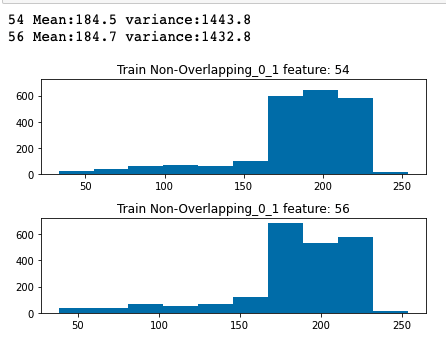
\includegraphics[scale=0.3]{../screenshot/train_non_over_01.png}

    \captionof{figure}{Image01 Non-Overlapping Test}
		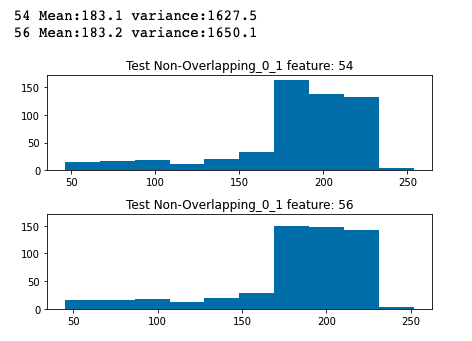
\includegraphics[scale=0.3]{../screenshot/test_non_over_01.png}

    \captionof{figure}{Image012 Non-Overlapping Train}
		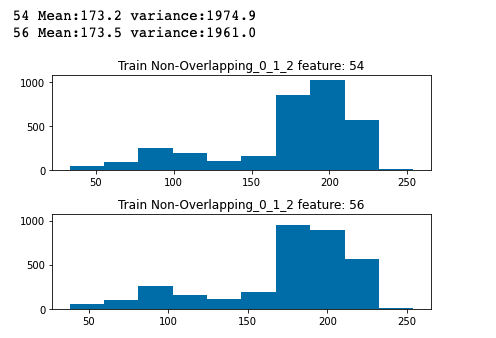
\includegraphics[scale=0.3]{../screenshot/train_non_over_012.png}

    \captionof{figure}{Image012 Non-Overlapping Test}
		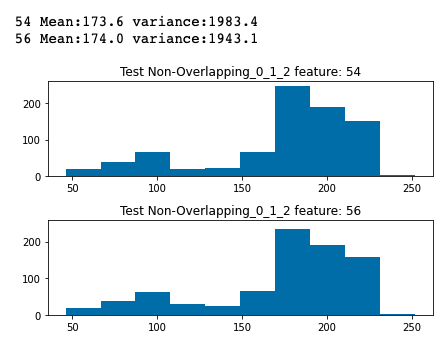
\includegraphics[scale=0.3]{../screenshot/test_non_over_012.png}

    \captionof{figure}{Image01 Overlapping Train}
		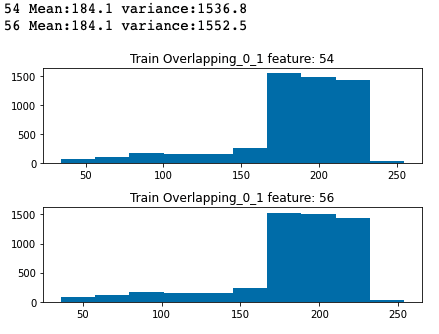
\includegraphics[scale=0.3]{../screenshot/train_over_01.png}

    \captionof{figure}{Image01 Overlapping Test}
		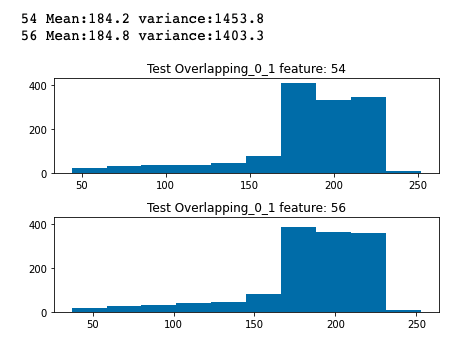
\includegraphics[scale=0.3]{../screenshot/test_over_01.png}

    \captionof{figure}{Image012 Overlapping Train}
		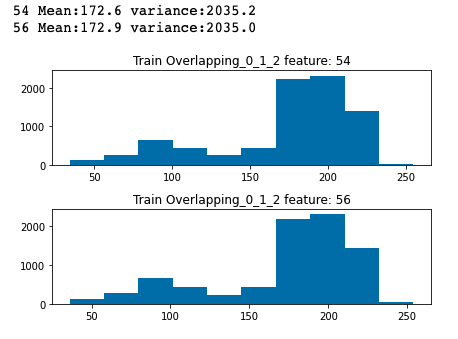
\includegraphics[scale=0.3]{../screenshot/train_over_012.png}

    \captionof{figure}{Image012 Overlapping Test}
		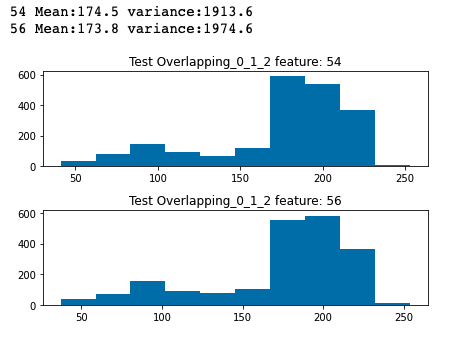
\includegraphics[scale=0.3]{../screenshot/test_over_012.png}
		
	\end{center}

  \hspace*{5mm} The scatterplot in 2.2 Figure 9 and Figure 10, represents the relationship of the black and white RGB color between features 54 and 56 of the train
  and test split dataset of the non-overlapping image01 dataset. Both features in the train and test split follow a similar positively correlated pattern.
  The data was also randomly distributed across all range of the black and white color spectrum. This suggests a great degree of randomness among the dataset.
  The non-overlapping image012 dataset in 2.2 Figure 11 and Figure 12 follow a positively linear pattern but deviated slightly from their test and train set. 
  In 2.2 Figure 11, image 2 had more of a cluster around the darker RGB values and image 0 and 1. This suggests that image 2 may contain a darker texture than that of
  image 0 and 1. This same pattern was also found in the test set. 

  \hspace*{5mm} In the overlapping dataset, 2.2 Figure 13 and Figure 14 of image01 showed that the relationship between feature 54 and 56 follow a positively linear pattern.
  The same pattern can be found in both the train and test set. Thus, the method of splitting the data into train and test did not destroy the original characteristics
  of the dataset and its integrity. Similarly, the overlapping plot of image012 in 2.2 Figure 15 and Figure 16, followed the same positively linear relationship
  between features 54 and 56. It also displayed similar characteristics to the non-overlapping dataset of image012 as image 2 had a large cluster on the darker RGB 
  values than that of image 0 and 1 due to its darker texture. This behavior was consistent through the non-overlapping and overlapping split, therefore, this suggests
  that the dataset was not altered to a large degree during its split. 

  \subsection{Figures Scatterplot} 
	\begin{center}
		\captionof{figure}{Image01 Train}
		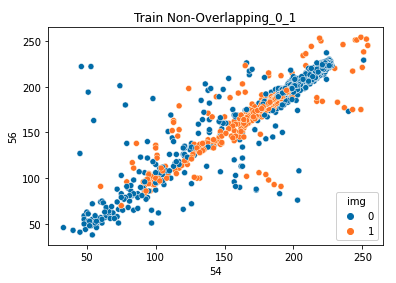
\includegraphics[scale=0.3]{../screenshot/train_scatter_non_over_01.png}

    \captionof{figure}{Image01 Test}
		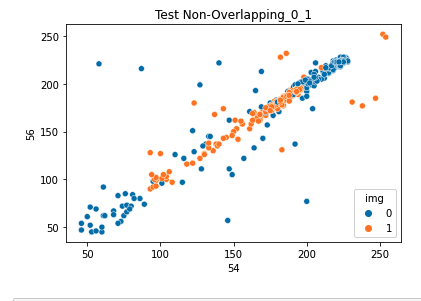
\includegraphics[scale=0.3]{../screenshot/test_scatter_non_over_01.png}

    \captionof{figure}{Image012 Train}
		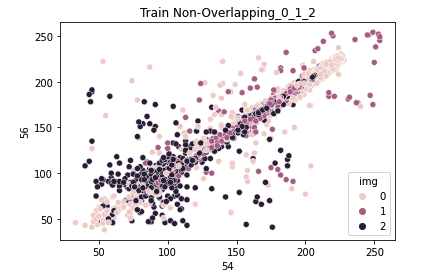
\includegraphics[scale=0.3]{../screenshot/train_scatter_nonover_012.png}

    \captionof{figure}{Image012 Test}
		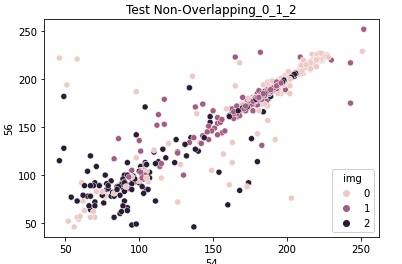
\includegraphics[scale=0.3]{../screenshot/test_scatter_nonover_012.png}

    \captionof{figure}{Image01 Train}
		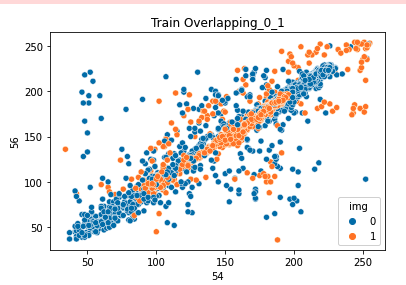
\includegraphics[scale=0.3]{../screenshot/train_scatter_over_01.png}

    \captionof{figure}{Image01 Test}
		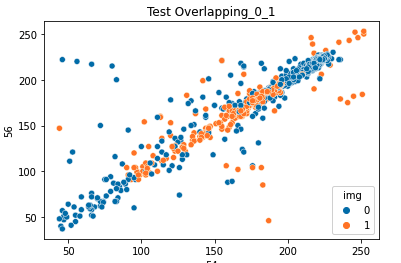
\includegraphics[scale=0.3]{../screenshot/test_scatter_01.png}

    \captionof{figure}{Image012 Train}
		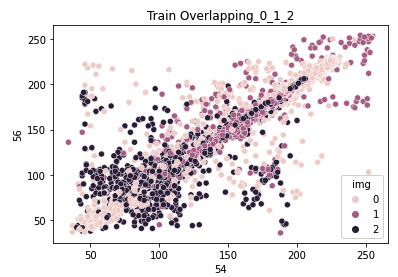
\includegraphics[scale=0.3]{../screenshot/train_scatter_012.png}

    \captionof{figure}{Image012 Test}
		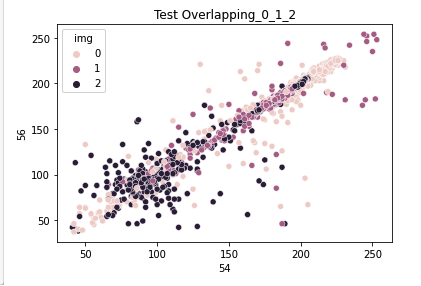
\includegraphics[scale=0.3]{../screenshot/test_scatter_012.png}
	\end{center}

  \section{Task 2}
  \hspace*{5mm}For task two, we're training the non-overlapping image01 and overlapping image01 on
  elastic net two class classifier model. This dataset represents a spanish pear and fuiji apple respectively.
  A function was created for this model by adding an L1 and L2 penalty function, so an input
  of trainx, trainy, testx and testy were only needed as input parameters to the function to
  yield a result. The resulting accuracy score and precission score was calculated manually based on the value shown
  in the presenting confusion matrix. Finally, feature selection was also used to increase the speed of the trained model
  and reduce the use of computational powers. 

  \hspace*{5mm} In the first elastic model, the data for non-overlapping image01 was used. The result of the model for
  non-overlapping image01 yielded a training accuracy of 0.69 and testing accuracy of 0.67 as shown in 3.1 Figure 17. A similar 
  score in both the train and test set indicate that the data was balanced between the train and test set. The confusion matrix in 3.1 
  Figure 18 indicate that there were 197 predictions of True Positive for class 0 and 175 predictions of True Positive for class 1. These
  results was then used to manually derived the accuracy and precision. According to the manual derivated result in 3.1 Figure 19, the overall
  accuracy of the model was 0.72 with a precision of 0.72 for class 0 and 0.72 for class 1. This accuracy score indicate that there was a sufficient
  number of true postives for class 0 and class 1. However, the number of false postives was still indicative in affecting the accuracy score.

  \subsection{Non-Overlapping Elastic-Net} 
  \begin{center}
    \captionof{figure}{Image01 Elastic-Net}
		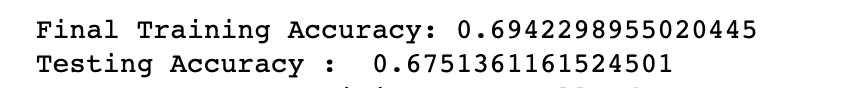
\includegraphics[scale=0.5]{../screenshot/Non-Overlapping-Elastic-results/results.png}

    \captionof{figure}{Image01 Elastic-Net Confusion-Matrix}
		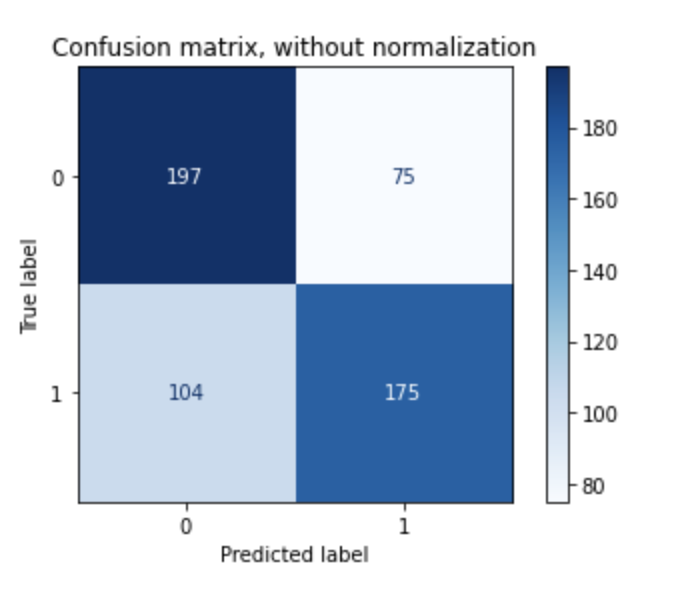
\includegraphics[scale=0.5]{../screenshot/Non-Overlapping-Elastic-results/cf.png}

    \captionof{figure}{Image01 Elastic-Net Derived Score}
		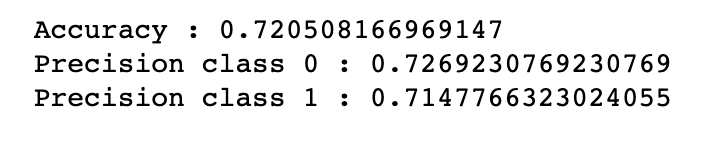
\includegraphics[scale=0.5]{../screenshot/Non-Overlapping-Elastic-results/calc_score.png}
  \end{center}


  \hspace*{5mm} In the second elastic model, the data for overlapping image01 was used. The result of the model for overlapping
  image01 resulted in a training accuracy of 0.60 and a testing accuracy of 0.59. This inidcated that the data had a great degree of
  randomeses and it was balanced in the train-test set. The confusion matrix in 3.2 Figure 21 resulted in 493 prediction of true prediction 
  and 314 of true prediction for class 0 and 1 respectively. However, in the derived precision score for class 0 was relatively lower than that
  of class 1 as shown in 3.2 Figure 22. This could indicate that there was an imbalance in the dataset between class 0 and class 1. Additionally, because of the nature of the
  image choosen, the black and white image of apple and pear had similar texture and texture. The overlapping nature of the dataset could distort the elastic-net loss function, 
  when it attempted to classify the two images. This also impacted the overall dervied accuracy score of the model with a value of 0.65 as shown in 
  3.2 Figure 23. An accuracy score of 0.65 indicate that this model was not sufficient enough for making a prediction. 

  \subsection{Overlapping Elastic-Net} 
  \begin{center}
    \captionof{figure}{Image01 Elastic-Net}
		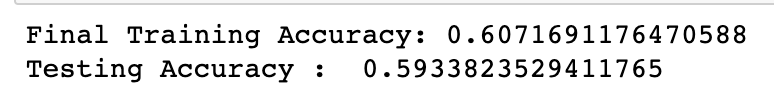
\includegraphics[scale=0.5]{../screenshot/Overlapping-Elastic-results/results.png}

    \captionof{figure}{Image01 Elastic-Net Confusion-Matrix}
		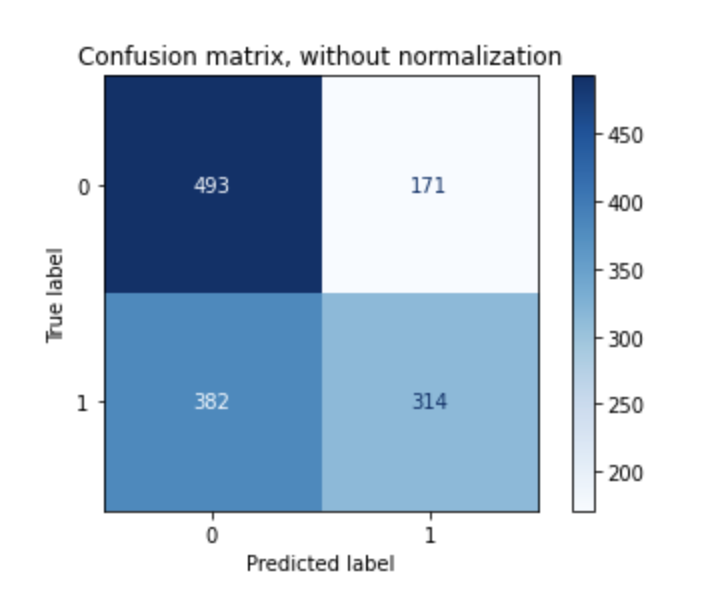
\includegraphics[scale=0.5]{../screenshot/Overlapping-Elastic-results/cf.png}

    \captionof{figure}{Image01 Elastic-Net Derived Score}
		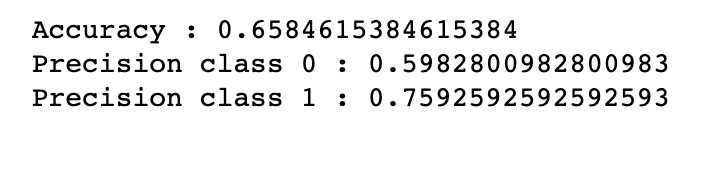
\includegraphics[scale=0.5]{../screenshot/Overlapping-Elastic-results/hand_score.png}
  \end{center}


  \section{Task 3}
  \hspace*{5mm} In Task 3, random forest classifier was used to classify the images of different set in non-overlapping image01, 
  overlapping image01, non-overlapping image012, and overlapping image012. Feature selection was also used in this model to increase
  the speed of the training time and reduce the computational power. The select from model feature selection from Sklearn compare the average
  importance of all features at a threshold value and dropped features that were below the threshold. 

  \hspace*{5mm} In the two class classification for non-overlapping image0 and image1, the training accuracy score was 0.95 and the testing 
  accuracy score was 0.92 based on 4.1 Figure 23. There was not a significant difference between the train and test score, this suggests that the train-test split 
  provided a well balanced data between the two classes. The confusion matrix in 4.1 Figure 24 confirmed a true prediction value of 240 and false prediction value of 
  32 for class 0 and a true prediction value of 269 and false prediction value of 10 for class 1. This indicate that the accuracy rate and the precision
  rate for class 0 and class 1 was relatively as seen in 4.1 Figure 25 of the derived accuracy score and precision for both class 0 and class 1 respectively.
  Class 0 had a precision rate of 0.92, while class 1 had a precision rate of 0.89. The random forest model, as a whole, performed better than the elastic
  net for classification of non-overlapping image01.

  \subsection{Non-Overlapping Random Forest} 
  \begin{center}
    \captionof{figure}{Image01 RF Score}
		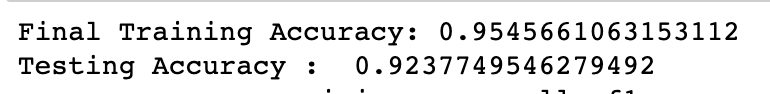
\includegraphics[scale=0.5]{../screenshot/Rf-Non-Overlapping01/score.png}

    \captionof{figure}{Image01 RF Confusion-Matrix}
		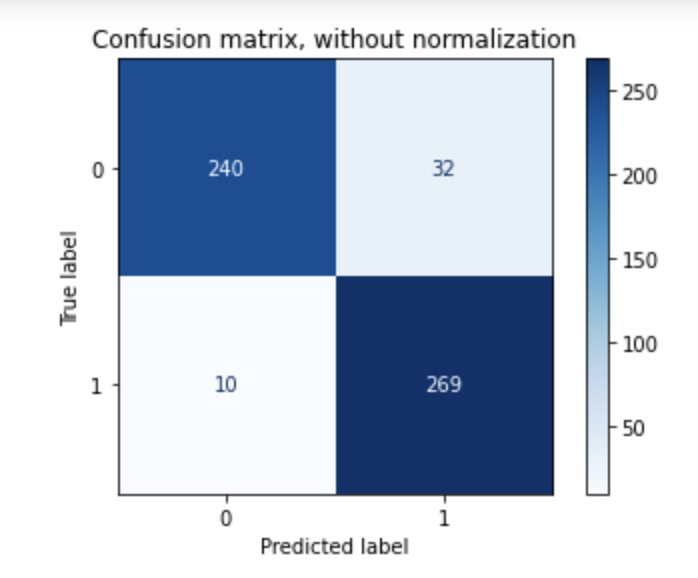
\includegraphics[scale=0.5]{../screenshot/Rf-Non-Overlapping01/cf.png}

    \captionof{figure}{Image01 RF Derived Score}
		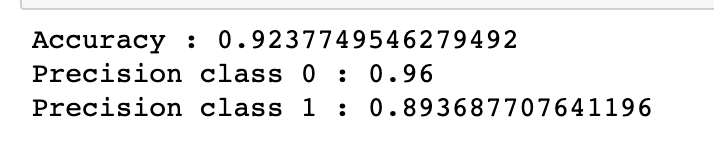
\includegraphics[scale=0.5]{../screenshot/Rf-Non-Overlapping01/hand_score.png}
  \end{center}


  \hspace*{5mm} For the overlapping two-class classificaiotn of image0 and image1, the training accruacy score was ~0.96 and the testing
  accuracy score was 0.92 based on 4.2 Figure 26. This small difference in accuracy score indicates that the train-test split provided an evenly balanced data for the test and train
  set for the random forest model. The confusion matrix on 4.2 Figure 27 provided the result of the test set as class 0 had 590 true prediction and 74 false prediction,
  while class 1 had 666 true prediction and 30 false prediction. This indicated a high precision value for both class 0 and class 1 because the model
  was able to make a prediction of the two images at a high accuracy rate. Based on the value of this confusion matrix, the hand calculation for accuracy score,
  precision for class 1 and precision for class 0 was derived. In 4.2 Figure 28, the accuracy score from the dervied calculation was 0.92 with a precision of 0.95 and 0.9
  for class 0 and class 1 respectively. Based on these high precision values, it indicated that this model can be produced the same results when test with another
  dataset of the same characteristics. This model also performed significantly better than the elstaic-net for two-class classification of overlapping
  image0 and image1. 

  \subsection{Overlapping Random Forest} 
  \begin{center}
    \captionof{figure}{Image01 RF Score}
		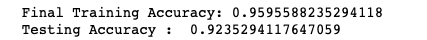
\includegraphics[scale=0.5]{../screenshot/Rf-Overlapping01/score.png}

    \captionof{figure}{Image01 RF Confusion-Matrix}
		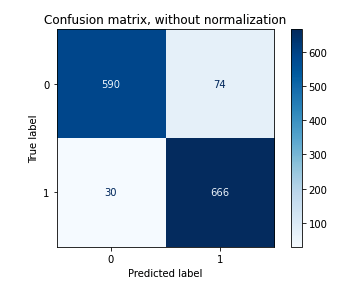
\includegraphics[scale=0.5]{../screenshot/Rf-Overlapping01/cf.png}

    \captionof{figure}{Image01 RF Derived Score}
		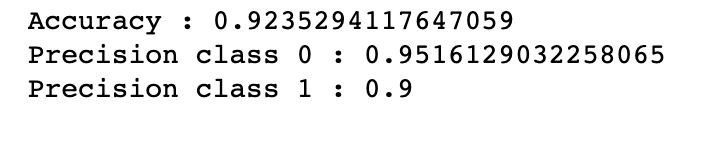
\includegraphics[scale=0.5]{../screenshot/Rf-Overlapping01/calc_score.png}
  \end{center}

  \hspace*{5mm} In contrast to the two-class non-overlapping classification, the three-class
  classification of image0, image1 and image2 testing and training accuracy score deviate in larger degree.
  In 4.3 Figure 29, the training accuracy for this model is 0.89, whereas the testing accuracy for this model is 
  0.78. This may indicate an overfit in the model and that the train-test split set did not generate a well balanced enough data.
  The confusion matrix in 4.3 Figure 30 showed that a true prediction value of 212 for class 0, 221 for class 1, and 212 for class 2.
  These values was then used to dervied the caculated precision for each of the class. 4.3 Figure 31 indicated that class 0 had a 0.89 precision,
  class 1 had a precision of 0.74 and class 2 ha da precision of 0.73. The difference in this precision score can suggest that the model
  was overfitted to favor class 0. 
  \subsection{Non-Overlapping Random Forest} 
  \begin{center}
    \captionof{figure}{Image012 RF Score}
		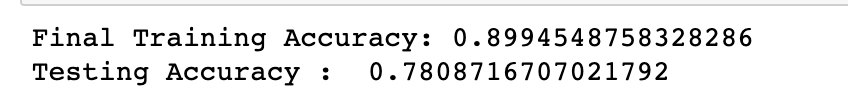
\includegraphics[scale=0.5]{../screenshot/Rf-Non-Overlapping012/score.png}

    \captionof{figure}{Image012 RF Confusion-Matrix}
		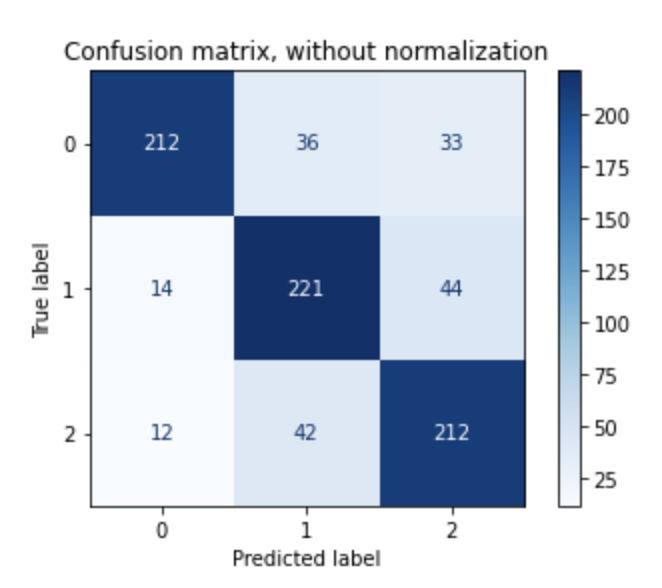
\includegraphics[scale=0.5]{../screenshot/Rf-Non-Overlapping012/cf.png}

    \captionof{figure}{Image012 RF Derived Score}
		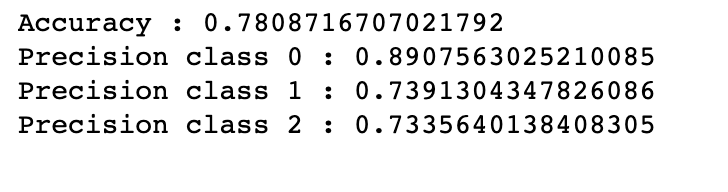
\includegraphics[scale=0.5]{../screenshot/Rf-Non-Overlapping012/calc_score.png}
  \end{center}


  \hspace*{5mm} Similar to the three-class non-overlapping random forest model, the three-class classification of overlapping 
  image0, image1 and image2 testing and training accuracy score also deviated to a noticeable extent.
  In 4.4 Figure 32, the training accuracy for this model is 0.91, whereas the testing accuracy for this model is 
  0.83. This may indicate a slight overfit in the model and that the train-test split set did not generate a well balanced enough data.
  The confusion matrix in 4.4 Figure 33 showed that a true prediction value of 552 for class 0, 608 for class 1, and 545 for class 2.
  These values was then used to dervied the caculated precision for each of the class. 4.4 Figure 34 indicated that class 0 had a 0.94 precision,
  class 1 had a precision of 0.77 and class 2 ha da precision of 0.81. The difference in this precision score can suggest that the model
  was overfitted to favor class 0, which is similar to that of the three-class random forest non-overlapping model. Although the dataset was 
  randomly shuffled, the training set may have contained slightly more data for class 0 than that of class 2 and class 1.  

  \subsection{Overlapping Random Forest} 
  \begin{center}
    \captionof{figure}{Image012 RF Score}
		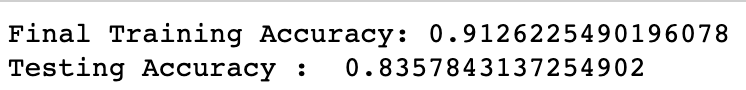
\includegraphics[scale=0.5]{../screenshot/Rf-Overlapping012/score.png}

    \captionof{figure}{Image012 RF Confusion-Matrix}
		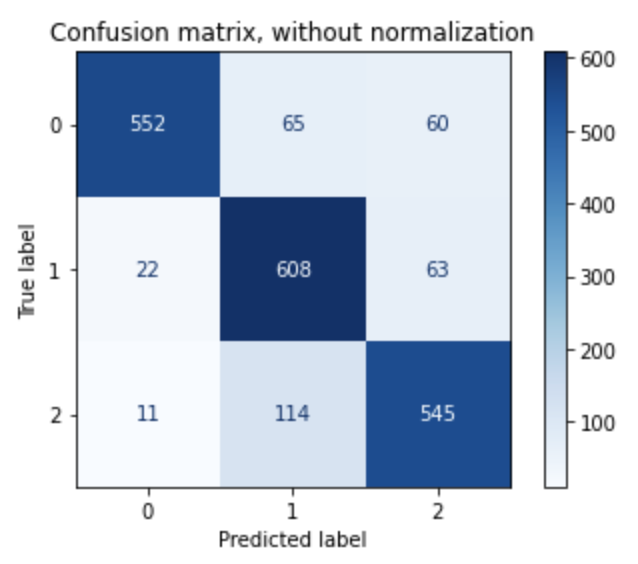
\includegraphics[scale=0.5]{../screenshot/Rf-Overlapping012/cf.png}

    \captionof{figure}{Image012 RF Derived Score}
		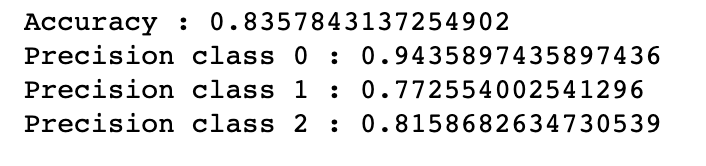
\includegraphics[scale=0.5]{../screenshot/Rf-Overlapping012/calc_result.png}
  \end{center}


\end{multicols*}

		

	

\end{document}